\chapter{Demonstrace použití knihovny}\label{chap:demonstration}

Tato kapitola popisuje ukázku použití nově vytvořené testovací knihovny.


\section{Predispozice ke spuštění testovací knihovny}\label{sec:test_requirements}

K tomu, aby mohla být testovací knihovna spuštěna, musí mít stroj nainstalované tyto položky:

\begin{itemize}
    \item Visual Studio 2022
    \item .NET 6
    \item Docker Desktop
\end{itemize}

Zároveň pro Docker Daemon, jenž je součástí Docker Desktop, musí být nastaveny rozmezí IP adres, ve kterých lze vytvářet sítě. To lze upravit v Docker Desktop v nastavení pod kolonkou \inlinecode{Docker Engine}. Možnou ukázku dodatečného nastavení můžeme vidět na výpisu \ref{listing:docker_conf}. 

\begin{listing}[htbp]
    \centering
    \begin{cminted}[breaklines,autogobble]{json}
"default-address-pools": [
    {
      "base": "172.17.0.0/12",
      "size": 20
    },
    {
      "base": "192.168.0.0/16",
      "size": 24
    }
]
    \end{cminted}
\caption{Nastavení rozmezí IP adres pro Docker}
\label{listing:docker_conf}
\end{listing}


\section{Definice testu}\label{sec:modbus_test}

Hlavní výhodou nové testovací knihovny je její flexibilita ve vytváření jednotlivých topologií ve virtualizovaném prostředí. Cílem tedy bylo navrhnout test, který by byl lehce škálovatelný a použitelný na všechny topologie. 

Nejdříve byl ovšem pro komunikaci zvolen průmyslový protokol ModbusTCP. Všechna komunikace mezi zařízeními tedy probíhá dle jeho specifikace. K úspěšné komunikaci tedy bude potřeba právě jeden server a alespoň jeden klient, který bude se serverem komunikovat. Test poté bude probíhat následovně:

\begin{enumerate}
    \item Uvnitř testovacího prostředí bude běžet server, který bude přijímat komunikaci.
    \item Klient přečte hodnotu registru, který je nazýván jako tzv. \textit{coil}, je na adrese 0 a má velikost právě jeden bit. Pokud je jeho hodnota rovna 0, poté se pokusí změnit jeho hodnotu na hodnotu 1. V případě neúspěchu je tento krok opakován.
    \item Klient přečte první čtyři tzv. \textit{holding} registry, které mají adresu 0-3. 
    \item Klient inkrementuje získanou hodnotu registrů. Pokud hodnota inkrementací překročí maximální povolenou hodnotu v registrech, je registr nastaven na hodnotu 0.
    \item Klient zapíše nové hodnoty zpátky do daných registrů.
    \item Klient znovu přečte hodnotu z daných registrů a zkontroluje, zda byly nové hodnoty správně zapsány.
    \item Klient nastaví registr, který nastavil v druhém kroku zpátky na hodnotu 0.
\end{enumerate}

Tento test je jednoduše škálovatelný na libovolný počet klientů. Každý klient bude provádět kroky 2 až 7. Je ale ovšem potřeba zajistit exkluzivní přístup k daným registrům, tedy pouze jeden klient může v danou chvíli manipulovat s danými holding registry. 

K tomu slouží krok 2 a 7, kdy coil registr na adrese 0 slouží jako zámek. Pokud je tento registr úspěšně nastaven na hodnotu 1, tak poté pouze tento klient, jenž tuto hodnotu nastavil, může zapisovat do daných registrů. V opačném případě bude požadavek na zápis odmítnut.

\section{Implementace testu}\label{sec:python_test_impl}

Implementace testu vyžaduje implementaci dvou zařízení - serveru a klienta. Jazykem implementace pro obě zařízení byl zvolen jazyk Python. Obě zařízení budou pro komunikaci využívat knihovnu pyModbusTCP. Tato knihovna obsahuje implementaci námi požadovaného průmyslového protokolu ModbusTCP, a to jak pro server, tak pro klienta.
 
\subsection{Server}

Na straně serveru je potřeba zajistit exkluzivní přístup pro jednotlivé klienty, tedy aby pouze jeden klient mohl manipulovat s registry. Knihovna pyModbusTCP definuje tyto tři třídy:

\begin{itemize}
    \item \inlinecode{ModbusServer} - logika serveru
    \item \inlinecode{DataBank} - třída, která uchovává data registrů a zajištuje bezpečný přístup k nim
    \item \inlinecode{DataHandler} - třída, která mapuje volání serveru na na metody třídy DataBank
\end{itemize}

Knihovna přímo podporuje použití vlastní implementace tříd \inlinecode{DataBank} a \inlinecode{DataHandler}. Třída \inlinecode{DataHandler} obsahuje pro zápis tyto dvě funkce:

\begin{itemize}
    \item \inlinecode{write\_coils} - zápis do coil registrů 
    \item \inlinecode{write\_h\_regs} - zápis do holding registrů
\end{itemize}

Do obou těchto funkcí byla přidána kontrola, zda má daný klient povolení zapisovat. To je kontrolováno za pomoci IP adresy. Funkce \inlinecode{write\_coils} ovšem dovoluje zapisovat i v případě, že registr na adrese 0 má hodnotu 0. Pokud je hodnota tohoto registru nastavena na 1, je poté uložena IP adresa zařízení, které danou změnu provedlo. Symetricky, pokud je hodnota téhož registru nastavena na hodnotu nula, tak poté je IP adresa smazána a je povolen zápis do coil registru dalšímu klientovi. Funkce zároveň obsahuje zámek pro zajištění exkluzivního přístupu při zamykání a odemykání. 

Logika třídy \inlinecode{DataBank} byla nepozměněna. Jedinou změnou byla implementace metod \inlinecode{on\_coils\_change} a \inlinecode{on\_holding\_registers\_change}, za jejichž pomoci je vypsána každá změna v příslušných registrech. 

\subsection{Klient}

Pro orchestraci musí být klient připojen k testovací službě. K tomu bude využita python implementace testovací knihovny, která obsahuje vše potřebné k vytvoření spojení a řízení zařízení na základě instrukcí od testovací služby. 

K umožnění testování je potřeba provést tyto věci:

\begin{enumerate}
    \item Definovat výčtový typ, jenž bude definovat test. Jeho číselná hodnota musí být stejná jak na zařízení, tak v testovacím projektu, kde poběží testovací knihovna.
    \item Implementovat testovací případ, který bude vycházet z abstraktní třídy \inlinecode{TestCase}.
    \item Vytvořit funkci, která po obdržení identifikátoru testu v argumentu funkce navrátí instanci testu, jenž daný identifikátor reprezentuje.
\end{enumerate}


V implementaci klienta výčtovým typem, který definuje testy, je třída \inlinecode{TestList}. Následně třída \inlinecode{TestModbusRead} definuje daný testovací případ. V neposlední řadě funkce \inlinecode{get\_test(int)} převádí identifikátor na instanci testovacího případu. 

Do souboru \inlinecode{main.py}, který je hlavním zdrojovým souborem programu, bylo také přidáno získání přepínačů programu, jež jsou získány prostřednictvím knihovny \inlinecode{argparse}. Program má tyto dva přepínače:

\begin{itemize}
    \item \inlinecode{-s}, \inlinecode{--service} - IP adresa nebo doména testovací služby
    \item \inlinecode{-p}, \inlinecode{--port} - port testovací služby
\end{itemize}

Program díky těmto přepínačům obdrží informace o tom, kde běží testovací služba, na kterou se při jejím spuštění připojí. Spuštění \inlinecode{TestRunner}, třídy, která se stará o běh zařízení, pak můžeme vidět na výpisu \ref{listing:server_main}. Jako první je běh inicializován za pomoci funkce \inlinecode{init}, díky čemuž proběhne inicializační fáze připojení se k testovací službě. 

Následně je zavolána funkce \inlinecode{handle\_instructions}, která čeká na instrukce od testovací služby a ty následně obsluhuje. Běh zařízení je ukončen po obdržení adekvátní zprávy o ukončení testování.

\begin{listing}[htbp]
    \centering
    \begin{minted}[breaklines,autogobble]{python}
args = args.parse_args()
testrunner = TestRunner(get_test)
testrunner.init(args.service, args.port)
testrunner.handle_instructions()
    \end{minted}
\caption{Spuštění řízení testovaného zařízení}
\label{listing:server_main}
\end{listing}


\subsection{Definice docker kontejnerů}

Díky podobné struktuře obou programů jsou všechny kontejnery skoro identické, až na možnou změnu v kopírování zdrojových souborů. Kontejnery vychází z předem definovaného obrazu \inlinecode{testlib-ubuntu-base}. Tento obraz je následně rozšířen o tyto balíčky:

\begin{itemize}
    \item \inlinecode{python-3.10}
    \item \inlinecode{python-3.10-venv}
\end{itemize}

Tyto balíčky jsou nutnou součástí kontejneru a slouží ke spuštění dříve definovaných Python programů. Následně je vytvořena složka \inlinecode{app}, do které jsou nakopírovány všechny zdrojové soubory programu. Spolu s ní je vytvořena složka \inlinecode{packages}, do které jsou nakopírovány všechny balíčky ze stejnojmenné složky v kořenové složce programu. Tato složka slouží pro balíčky, které nebyly uveřejněny a tedy nejsou dostupné z veřejného repozitáře.

Po nakopírování všech souborů je vytvořeno virtuální Python prostředí. S jeho pomocí jsou poté nainstalovány všechny lokální balíčky ve složce packages, pokud nějaké existují. Poté jsou nainstalovány všechny balíčky obsažené v souboru \inlinecode{requirements.txt}. Ten obsahuje seznam všech potřebných balíčků ke spuštění programu, včetně těch, jež nejsou veřejně dostupné. Pokud je možné program spustit bez argumentů, tak je do kontejneru přidán i příkaz na spuštění aplikace. Při použití v knihovně ovšem bude toto spuštění změněno. Ukázku definice docker kontejneru můžeme vidět na výpise \ref{listing:dockerfile}

\begin{listing}[htbp]
    \centering
    \begin{cminted}[breaklines,autogobble, fontsize=\footnotesize]{dockerfile}
FROM wheeeper/testlib-ubuntu-base:22.04 AS base
RUN apt-get update && apt-get upgrade -y
RUN apt-get update && apt-get install -y python3.10 python3.10-venv
WORKDIR /app
COPY "src/" "/app/src"
COPY ["main.py", "requirements.txt", "/app/"]

RUN mkdir /packages
COPY "./packages/" "/packages/"
RUN python3.10 -m venv /opt/venv

RUN /opt/venv/bin/pip install  /packages/** || true
RUN /opt/venv/bin/pip install -r /app/requirements.txt 
CMD ["/opt/venv/bin/python", "/app/main.py"]
    \end{cminted}
\caption{Ukázka definice kontejneru}
\label{listing:dockerfile}
\end{listing}

\subsection{Definice virtualizovaného prostředí}

Ke spuštění zařízení ve virtualizovaném prostředí je potřeba definovat nastavení virtualizovaného prostředí, jež bylo popsáno v sekci \ref{sec:env_conf}. K testování na všech třech požadovaných topologiích budou potřeba minimálně tři konfigurace, které ovšem budou v mnoha částech podobné. První položkou v konfiguraci jsou označení virtualizovaného prostředí. Ty dle topologie budou:

\begin{itemize}
    \item \inlinecode{modbus\_line} - konfigurace s topologií sériové linky
    \item \inlinecode{modbus\_star} - konfigurace s topologií hvězdy
    \item \inlinecode{modbus\_circle} - konfigurace s topologií kruhu
\end{itemize}

Poté následuje konfigurace počtu očekávaných zařízení. Každá konfigurace bude obsahovat 1 server a 6 klientů. K testovací službě budou připojeni pouze klienti, tedy testovací služba bude očekávat 6 zařízení. Ukázku konfigurace obou položek můžeme vidět na výpisu \ref{listing:conf_devices}

Další položkou v konfiguraci jsou jednotlivá zařízení. Definici jednotlivých zařízení můžeme vidět na výpisu \ref{listing:conf_devices}. Virtualizované prostředí obsahuje dle definice dva typy zařízení - server a klienty. Server je definován pod názvem \inlinecode{modbus\_server}, je typu \inlinecode{default} a je definován v \inlinecode{..\textbackslash server\textbackslash Dockerfile}. V kolonce \inlinecode{commands} pak můžeme vidět příkaz na spuštění zařízení. Server má také nastavenu kolonku \inlinecode{logging} na hodnotu \inlinecode{true}, čímž bude zaručeno zaznamenávání komunikace mezi serverem a klienty.

Následně lze vidět definice klientů. Ti jsou pojmenování jakožto \inlinecode{modbus\_client\_[1-6]}. Každá definice klienta je totožná a liší se pouze v názvu zařízení. Klient je definován v \inlinecode{..\textbackslash client\textbackslash Dockerfile} a je taktéž typu default. V kolonce \inlinecode{commands} pak lze vidět příkaz na spuštění zařízení, kde v přepínačích jsou předány parametry pro připojení se k testovací službě.


\begin{listing}[htbp]
    \centering
    \begin{minted}[breaklines,autogobble, fontsize=\footnotesize]{yaml}
label: modbus_(line|star|circle)
service:
  connections: 6
containers:
    modbus_server:
      build: 
          dockerfile: ..\server\Dockerfile
      type: default
      commands:
        - "/opt/venv/bin/python /app/main.py"
      logging: true
    modbus_client_1:
      build: 
          dockerfile: ..\client\Dockerfile
      type: default
      commands:
        - "/opt/venv/bin/python /app/main.py -s host.docker.internal -p 1337"
        .
        .
        .
    modbus_client_6:
      build: 
          dockerfile: ..\client\Dockerfile
      type: default
      commands:
        - "/opt/venv/bin/python /app/main.py -s host.docker.internal -p 1337"
    \end{minted}
\caption{Nastavení zařízení v konfiguraci virtualizovaného prostředí}
\label{listing:conf_devices}
\end{listing}

V neposlední řadě je potřeba nadefinovat kolonku \inlinecode{links}, která definuje propojení mezi zařízeními. Definice pro všechny topologie můžeme vidět na výpisu \ref{listing:conf_links}. Jak je vidět, definice je jednoduchá, intuitivní a každá položka v seznamu definuje právě jedno spojení.

\begin{listing}[htbp]
    \centering
    \begin{cminted}[breaklines,autogobble, fontsize=\footnotesize]{yaml}
# Definice topologie seriové linky
links:
- "modbus_server:modbus_client_1"    
- "modbus_client_1:modbus_client_2"    
- "modbus_client_2:modbus_client_3"    
- "modbus_client_3:modbus_client_4"    
- "modbus_client_4:modbus_client_5"    
- "modbus_client_5:modbus_client_6"

# Definice topologie hvězdy
links:
- "modbus_server:modbus_client_1"    
- "modbus_server:modbus_client_2"    
- "modbus_server:modbus_client_3"    
- "modbus_server:modbus_client_4"    
- "modbus_server:modbus_client_5"    
- "modbus_server:modbus_client_6"

# Definice topologie kruhu
links:
- "modbus_server:modbus_client_1"    
- "modbus_client_1:modbus_client_2"    
- "modbus_client_2:modbus_client_3"    
- "modbus_client_3:modbus_client_4"    
- "modbus_client_4:modbus_client_5"    
- "modbus_client_5:modbus_client_6"
- "modbus_client_6:modbus_server"
    \end{cminted}
\caption{Nastavení propojení zařízení pro všechny topologie}
\label{listing:conf_links}
\end{listing}

\section{Testovací projekt}

K tomu, aby mohla být spuštěna testovací knihovna, je zapotřebí vytvořit testovací projekt. Tento projekt musí obsahovat vytvořenou testovací knihovnu a také testovací knihovny MSTest. Projekt je možné vytvořit ze šablon, jenž jsou poskytnuty IDE Visual Studio 2022\cite{vs2022}. K vytvoření projektu byla použita šablona s názvem \textit{MSTest Test Project}. Do vytvořeného projektu je následně přidána testovací knihovna prostřednictvím správce balíčků NuGet\cite{nuget}. 

Aby mohl program využívat relativních cest pro všechny cesty konfigurační soubory, je potřeba nakopírovat všechny potřebné soubory do výstupní složky kompilace. K tomu byla do projektového souboru přidána direktiva na zkopírování složky \inlinecode{virtual\_env}, která obsahuje všechny potřebné zdroje. Tuto direktivu můžeme vidět na výpisu \ref{listing:copy_virtual_env}

\begin{listing}[htbp]
    \centering
    \begin{cminted}[breaklines,autogobble, fontsize=\footnotesize]{xml}
<ItemGroup>
    <Content Include="virtual_env\**">
        <CopyToOutputDirectory>PreserveNewest</CopyToOutputDirectory>
    </Content>
</ItemGroup>
    \end{cminted}
\caption{Direktiva pro zkopírovaní složky při kompilaci}
\label{listing:copy_virtual_env}
\end{listing}


Po přidání testovací knihovny je potřeba zajistit její inicializaci a také její správné ukončení. Tuto definici lze vidět na výpisu \ref{listing:lib_init}. Tento proces zůstal nepozměněn od původní testovací knihovny. Jak je vidět, pro obě operace existují separátní funkce, které obsahují adekvátní atributy \inlinecode{AssemblyInitialize}, respektive \inlinecode{AssemblyCleanup}. Následně testovací knihovna MSTest zajistí jejich spuštění před započetím testování a po ukončení testovaní.  

\begin{listing}[htbp]
    \centering
    \begin{cminted}[breaklines,autogobble, fontsize=\small]{csharp}
[TestClass]
public static class TestLibInit
{
    [AssemblyInitialize()]
    public static void AssemblyInit(TestContext context)
    {
        TestLib.API.AssemblyInit(Assembly.GetExecutingAssembly());
    }

    [AssemblyCleanup()]
    public static void AssemblyCleanup()
    {
        TestLib.API.AssemblyCleanup();
    }
}
    \end{cminted}
\caption{Inicializace a ukončení testovací knihovny}
\label{listing:lib_init}
\end{listing}

Následně je zapotřebí definovat výčtový typ, který bude reprezentovat jednotlivé testy. Testovací knihovna požaduje, aby každý výčtový typ obsahoval atribut \inlinecode{TestEnum}. Díky němu může všechny výčtové typy identifikovat a následně kontrolovat kolize mezi jejich číselnými hodnotami. Definici výčtového typy můžeme vidět na výpisu \ref{listing:test_enum}. 

\begin{listing}[htbp]
    \centering
    \begin{cminted}[breaklines,autogobble, fontsize=\small]{csharp}
[TestEnum]
public enum TestCaseE
{
    TEST_SUCCESS = 0,
    MODBUS_READ = 10,
    TEST_IPERF = 6969
};
    \end{cminted}
\caption{Definice výčtového typu který identifikuje jednotlivé testy}
\label{listing:test_enum}
\end{listing}

Jak je vidět, výčtový typ obsahuje tři testy:

\begin{itemize}
    \item \inlinecode{TEST\_SUCCESS} - úspěšný test, který ve všech fázích navrátí hodnotu \inlinecode{true}
    \item \inlinecode{MODBUS\_READUPDATE} - test definovaný v sekci \ref{sec:modbus_test}
    \item \inlinecode{TEST\_IPERF} - test na měření výkonu, jenž je popsán v sekci \ref{sec:perfomance_test}
\end{itemize}

Nyní zbývá jednotlivé třídy dle konvencí testovací knihovny MSTest. Pro každou topologii vytvoříme testovací třídu. Jednotlivé testy v daných třídách budou probíhat na v jednotném virtualizovaném prostředí. Ukázku definice pro topologii sériové linky můžeme vidět na výpisu \ref{listing:test_class}. Jako první je definována metoda \inlinecode{StartUp}. Tato metoda je opatřena atributem \inlinecode{ClassInitialize}, který zaručí její zavolání před spuštěním všech testů ve třídě. Následně za pomoci metody \inlinecode{API.BuildEnvironment} je inicializováno dané virtualizované prostředí, kdy v argumentu metoda obdrží cestu ke konfiguračnímu souboru.

Následně je zde metoda \inlinecode{TestReadAndUpdate}, která definuje námi požadovaný test. Tato metoda je opatřena atributem \inlinecode{TestMethod}. Uvnitř metody je následně zavolána metoda \inlinecode{API.Run}, kdy v argumentu je předán identifikátor testu. 

\begin{listing}[htbp]
    \centering
    \begin{cminted}[breaklines,autogobble, fontsize=\footnotesize]{csharp}
[TestClass]
public class ModbusLine
{
    [ClassInitialize]
    public static void StartUp(TestContext ctx)
    {
        API.BuildEnvironment(@"virtual_env\modbus\topologies\modbus-line.yaml");
    }

    [TestMethod]
    public void TestReadAndUpdate()
    {
        API.Run(TestCaseE.MODBUS_READUPDATE);
    }
}
    \end{cminted}
\caption{Ukázka definice testovací třídy}
\label{listing:test_class}
\end{listing}


\section{Spuštění testů}

Jednotlivé testy lze spustit přímo z IDE Visual Studio 2022\cite{vs2022}. Po zobrazení okna \textit{Test Explorer} lze vidět všechny testy dostupné v projektu. Ty lze následně ze stejného pohledu i spustit. Po dokončení je následně vidět, zda test proběhl úspěšně nebo ne. Pohled po úspěšném dokončení všech testů můžeme vidět na obrázku \ref{fig:modbus_test_success}. 

\begin{figure}[htbp]
    \centering 
    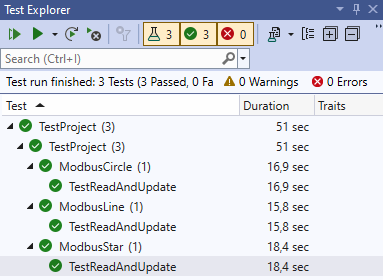
\includegraphics{assets/img/modbus_test.png}
    \caption{Pohled při úspěšném dokončení všech testů}
    \label{fig:modbus_test_success}
\end{figure}

Po každém testovacím běhu lze v kořenové složce programu nalézt složku se záznamem běhu všech testů. Uvnitř této složky jsou složky dle názvů všech virtualizovaných zařízení, které byly během testování použity. Tyto složky mají název dle kolonky \inlinecode{label} v konfiguraci. 

Uvnitř každé složky jsou poté složky s názvy jednotlivých zařízení. Složka je vytvořena právě tehdy, pokud je co ze zařízení uložit, jako například záznam výpisu ze zařízení. V jednotlivých složkách odposlouchávačů komunikace poté nalezneme i záznam komunikace v průběhu testu. 

Výstup ze serveru můžeme vidět na výpisu \ref{listing:modbus_server_log}. Pro kompaktnost z něj byla odstraněna informace o datu a času zápisu dané zprávy. Jak je vidět, všechna zařízení úspěšně provedla změnu a vždy pouze jeden klient prováděl danou změnu.

\begin{listing}[htbp]
    \centering
    \begin{cminted}[breaklines,autogobble, fontsize=\footnotesize]{text}
Modbus server started
change in coil space [False > True ] at @ 0x0000 from ip: 172.16.16.82   
change in hreg space [14671 > 14672] at @ 0x0000 from ip: 172.16.16.82   
change in hreg space [36946 > 36947] at @ 0x0001 from ip: 172.16.16.82   
change in hreg space [20782 > 20783] at @ 0x0002 from ip: 172.16.16.82   
change in hreg space [56603 > 56604] at @ 0x0003 from ip: 172.16.16.82   
change in coil space [True  > False] at @ 0x0000 from ip: 172.16.16.82   
change in coil space [False > True ] at @ 0x0000 from ip: 172.16.16.51   
change in hreg space [14672 > 14673] at @ 0x0000 from ip: 172.16.16.51   
change in hreg space [36947 > 36948] at @ 0x0001 from ip: 172.16.16.51   
change in hreg space [20783 > 20784] at @ 0x0002 from ip: 172.16.16.51   
change in hreg space [56604 > 56605] at @ 0x0003 from ip: 172.16.16.51   
change in coil space [True  > False] at @ 0x0000 from ip: 172.16.16.51   
change in coil space [False > True ] at @ 0x0000 from ip: 172.16.16.35   
change in hreg space [14673 > 14674] at @ 0x0000 from ip: 172.16.16.35   
change in hreg space [36948 > 36949] at @ 0x0001 from ip: 172.16.16.35   
change in hreg space [20784 > 20785] at @ 0x0002 from ip: 172.16.16.35   
change in hreg space [56605 > 56606] at @ 0x0003 from ip: 172.16.16.35   
change in coil space [True  > False] at @ 0x0000 from ip: 172.16.16.35   
change in coil space [False > True ] at @ 0x0000 from ip: 172.16.16.66   
change in hreg space [14674 > 14675] at @ 0x0000 from ip: 172.16.16.66   
change in hreg space [36949 > 36950] at @ 0x0001 from ip: 172.16.16.66   
change in hreg space [20785 > 20786] at @ 0x0002 from ip: 172.16.16.66   
change in hreg space [56606 > 56607] at @ 0x0003 from ip: 172.16.16.66   
change in coil space [True  > False] at @ 0x0000 from ip: 172.16.16.66   
change in coil space [False > True ] at @ 0x0000 from ip: 172.16.16.74   
change in hreg space [14675 > 14676] at @ 0x0000 from ip: 172.16.16.74   
change in hreg space [36950 > 36951] at @ 0x0001 from ip: 172.16.16.74   
change in hreg space [20786 > 20787] at @ 0x0002 from ip: 172.16.16.74   
change in hreg space [56607 > 56608] at @ 0x0003 from ip: 172.16.16.74   
change in coil space [True  > False] at @ 0x0000 from ip: 172.16.16.74   
change in coil space [False > True ] at @ 0x0000 from ip: 172.16.16.42   
change in hreg space [14676 > 14677] at @ 0x0000 from ip: 172.16.16.42   
change in hreg space [36951 > 36952] at @ 0x0001 from ip: 172.16.16.42   
change in hreg space [20787 > 20788] at @ 0x0002 from ip: 172.16.16.42   
change in hreg space [56608 > 56609] at @ 0x0003 from ip: 172.16.16.42   
change in coil space [True  > False] at @ 0x0000 from ip: 172.16.16.42   
    \end{cminted}
\caption{Výstup na serveru po testu}
\label{listing:modbus_server_log}
\end{listing}

Jak již bylo ukázáno u předchozí testovací knihovny\cite{bakalarka}, takto nastavený projekt lze poté spustit prostřednictvím Azure DevOps a tím zcela automatizovat testovaní. Jednotlivé testy lze přiřadit k testovacím příkazům definovaným v Azure DevOps, a ty se poté dají dle libosti spouštět. Je ovšem samozřejmé, že daný stroj, na kterém testování poběží, musí splňovat podmínky definované v sekci \ref{sec:test_requirements}.

